\section{Inverted Double Pendulum model} 
\begin{figure}[H]
	\centering
	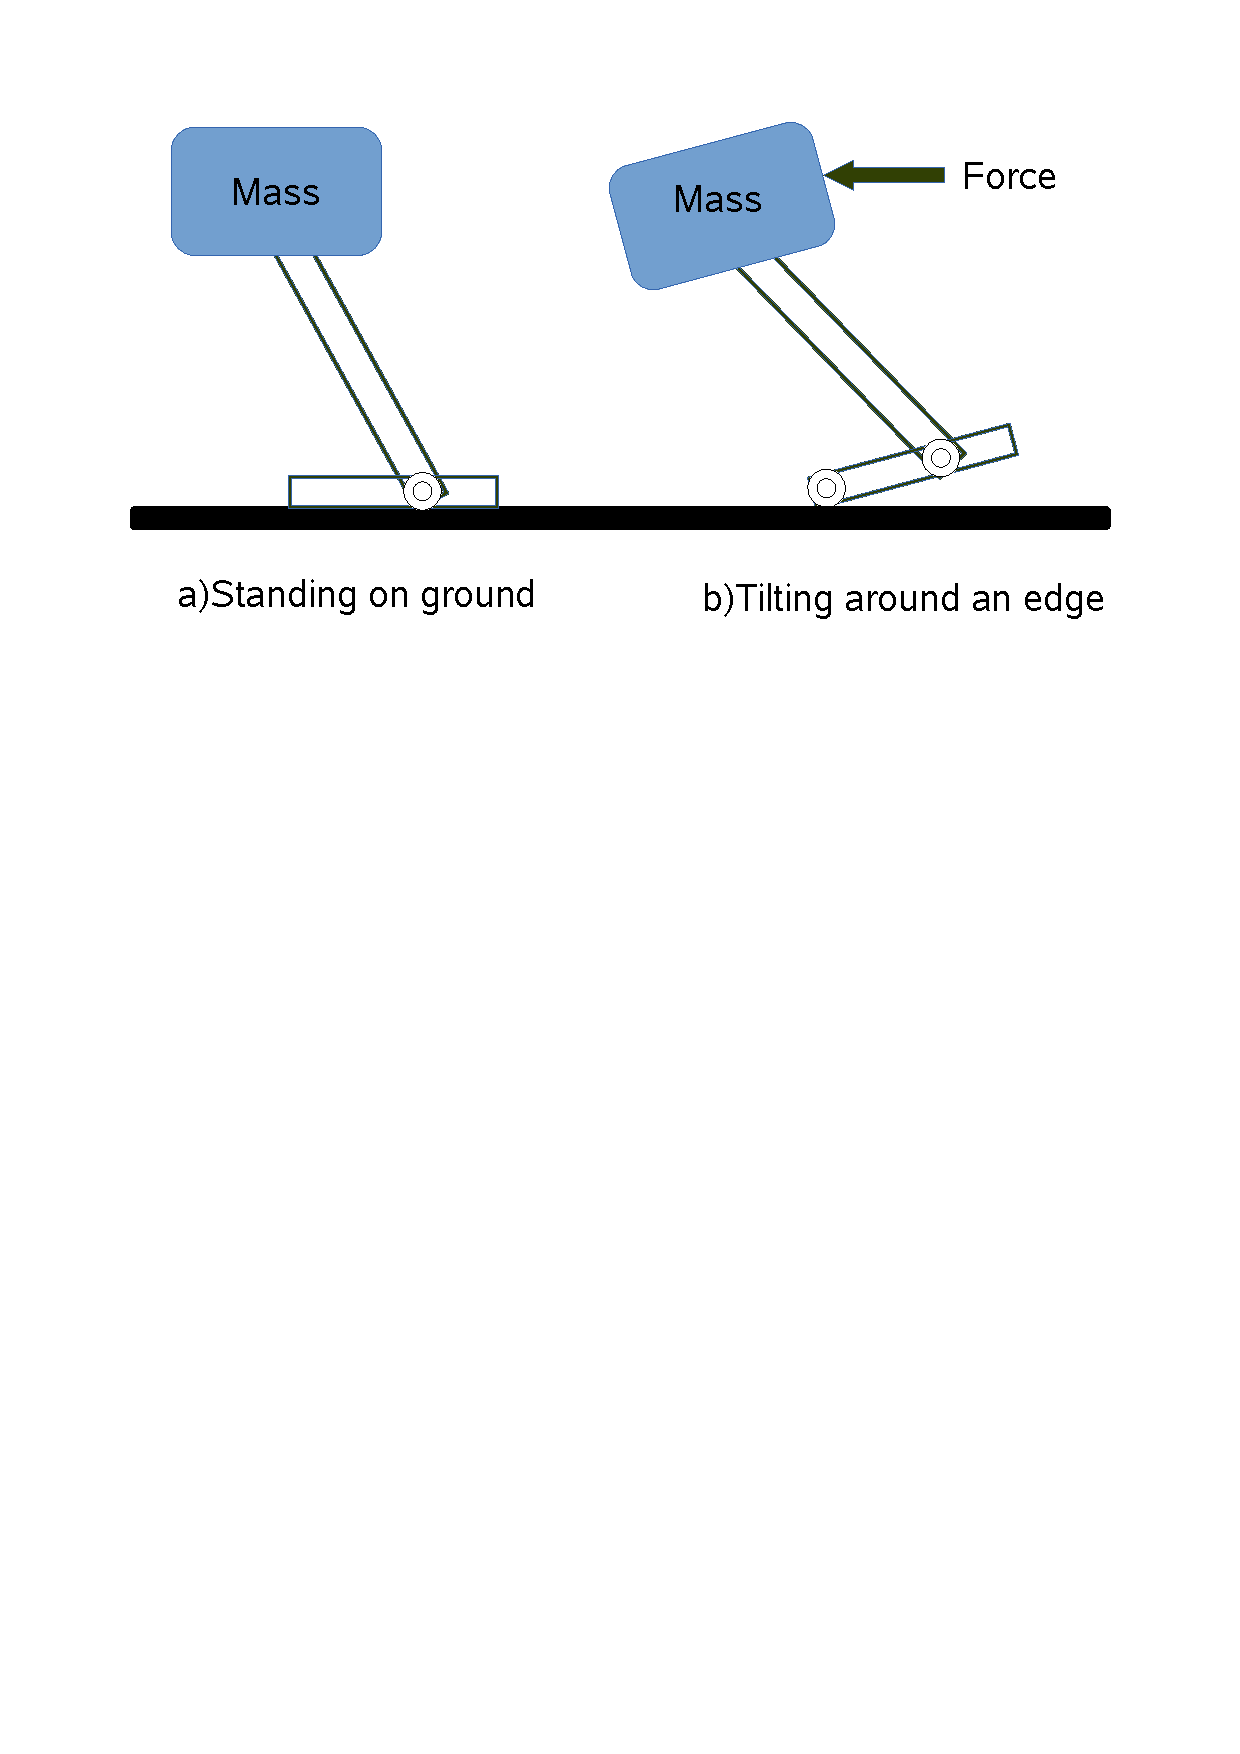
\includegraphics[trim = 0mm 180mm 0mm 10mm, scale=0.50]{Bilder/simp_uactcase.pdf}
	\caption{A simplified humanoid robot standing on one foot}
	\label{fig:idp_scene}
\end{figure}
At first to check the feasibility of solving the state estimation problem with the available measurements, a preliminary sub-problem is formulated. Since we are interested in estimating the under-actuated degrees of freedom, we have to consider the scenario where these under-actuated degrees of freedom are action on the robot. Let us consider the scenario where the robot is tilting around an edge of the foot by applying some external force as shown in Figure \ref{fig:idp_scene}.b. All the joints other than the ankle joint of the robot are assumed to remain static(joints does not produce any motion) throughout the experiment. The kinematics of \emph{Toro} is shown in Figure \ref{fig:toro_kin} is simplified to one joint on the ankle connecting the whole body with the foot as shown in \ref{fig:idp_scene}.a. The mass block in the Figure \ref{fig:idp_scene} represents the inertia of the upper body. The inertia of the leg is incorporated in the link connecting upperbody and foot. 

When the robot is tilting around an edge of the foot as shown in Figure \ref{fig:idp_scene}.b, we assume there is an imaginary joint located at the edge of the foot around which the robot tilts. Figure \ref{fig:idp_scene}.b resembles an inverted double pendulum in Figure \ref{fig:idp}.
\begin{figure}[H]
	\centering
	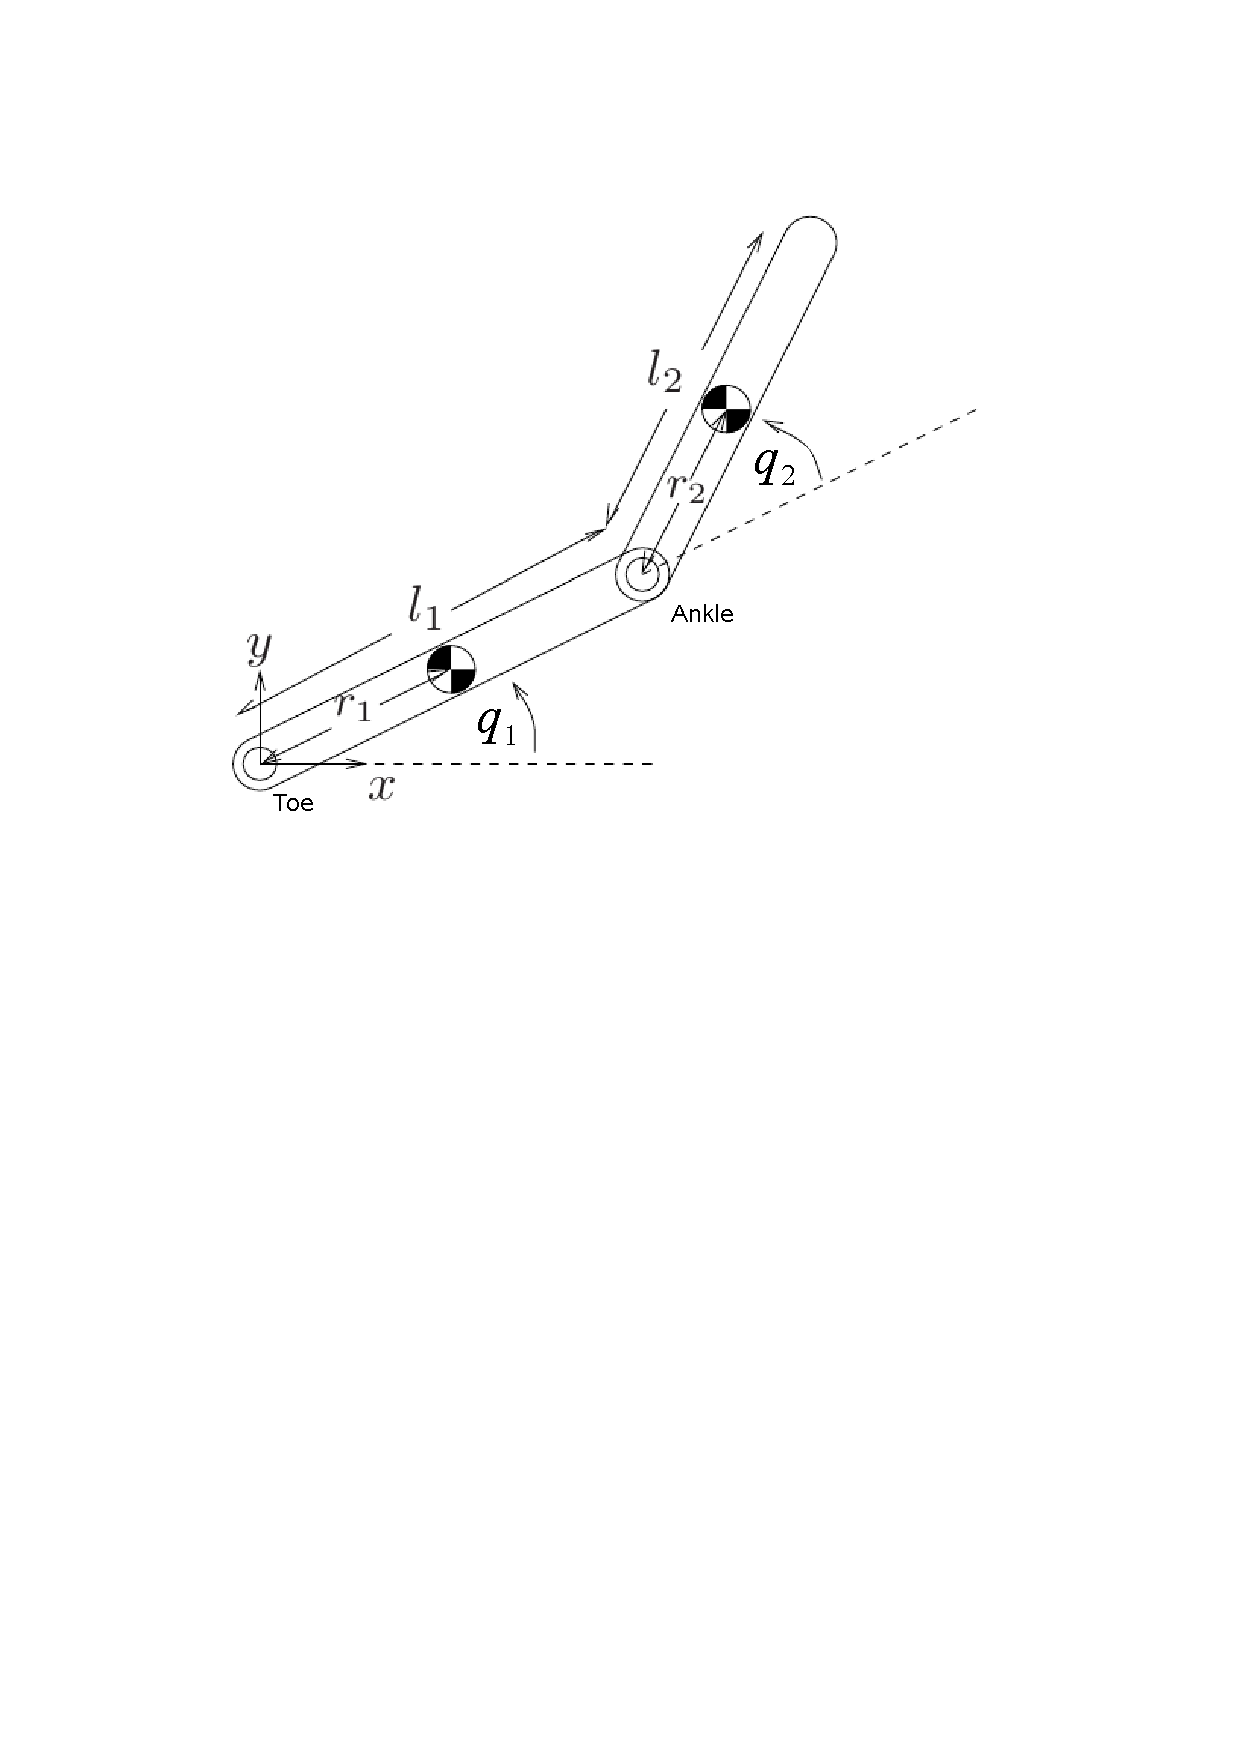
\includegraphics[trim= 0mm 145mm 0mm 0mm,clip, scale=0.65]{Bilder/inv_db_pend.pdf}
%	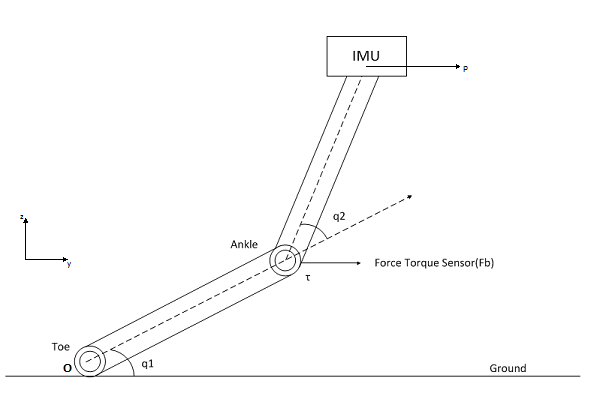
\includegraphics[scale=0.75]{Bilder/doublePendulum1.png}
	\caption[Inverted Double Pendulum]{Inverted Double Pendulum}
	\label{fig:idp}
\end{figure}
%\footnotetext{Image source: A mathematical introduction to robotic manipulation \cite[Chapter 4, Page 164]{mur94}}
 The inverted double pendulum shown in Figure \ref{fig:idp} consists two links of length $l_1$ and $l_2$. The distance between center of mass of link 1 from the toe joint is $r_1$, $r_2$ is the distance between center of mass of link 2 from the ankle joint. In the inverted pendulum model the ankle joint is actuated but the toe joint is unactuated. The degrees of freedom of this model are toe and ankle. Toe is the under-actuated degree of freedom whose motion parameters such as angle $q_1$ and angular velocity $\dot{q}_1$ needs to be estimated. The motion parameters of the inverted double pendulum are 
\begin{equation}
	 q = 
	\begin{bmatrix}
		q_{1}\\
		q_{2}
	\end{bmatrix}
	\hspace{2cm}
	 \dot{q} = 
	\begin{bmatrix}
		\dot{q_{1}}\\
		\dot{q_{2}}
	\end{bmatrix},
\end{equation}
where \emph{q} is the vector of joint angles and $\dot{q}$ is the vector of joint angular velocities. The angle $q_1$ and angular velocity $\dot{q}_1$ are the motion parameters of toe joint. Likewise $q_2$ and $\dot{q}_2$ are the motion parameters of ankle joint. The control input or torque applied to the ankle joint is $\tau$. 

The equation of motion of the inverted double pendulum is derived using Lagrange formulation given in Equation \ref{eq:lagrange}. The generalized coordinates of the system are $q_1$ and $q_2$, the velocities of the corresponding generalized coordinates are $\dot{q_1}$ and $\dot{q_2}$ as shown in Figure \ref{fig:idp}. The equation of motion of double pendulum written in general formulation of multi body system in Equation \ref{eq:dyn_mul_bdy} is
\begin{equation}
   \label{eq:dyn_idp}
	M(q_1,q_2)
	\begin{bmatrix}
		\ddot{q_{1}} \\
		\ddot{q_{2}} 
	\end{bmatrix}
	+ C(q_1,q_2,\dot{q}_1,\dot{q}_2)
    \begin{bmatrix}
		\dot{q_{1}} \\
		\dot{q_{2}} 
	\end{bmatrix}
	+ g(q_1,q_2) = 
    \begin{bmatrix} 0 \\ \tau \end{bmatrix},
\end{equation}
where, $M(q_1,q_2)$ represents the inertia matrix of the inverted double pendulum system. It is given by 
$$ M(q_1,q_2) = \begin{bmatrix}\
    \alpha+2\beta cos(q_2) & \delta + \beta cos(q_2) \\ 
    \delta + \beta cos(q_2) & \delta  \end{bmatrix},$$ where the terms $\alpha, \beta, \delta$ is given by
    $$
    \begin{aligned}
    \alpha &= \frac{1}{12} m_1 l_1^2 + \frac{1}{12} m_2 l_2^2 + m_1 r_1^2 + m_2 (r_2^2 + l_1^2),\\
    \beta &= m_2 l_1 r_2, \\
    \delta &= \frac{1}{12} m_2 l_2^2 + m_2 r_2^2.
    \end{aligned}
    $$
$C(q_1,q_2,\dot{q}_1,\dot{q}_2)$ represents the Coriolis matrix of the system. It is given by 
$$C(q_1,q_2,\dot{q}_1,\dot{q}_2) = 
\begin{bmatrix}
-\beta sin(q_2) \dot{q}_2 &-\beta sin(q_2)(\dot{q}_1 + \dot{q}_2) \\
-\beta sin(q_2) \dot{q}_1 & 0
\end{bmatrix},
$$
where $\beta$ is given in the previous equation. The gravity vector is represented by $g(q_1,q_2)$. It is given by
$$g(q_1,q_2) = 
\begin{bmatrix}
(m_1 r_1 +m_2 l_1)a_g cos(q_1) + m_2 r_2 a_g cos(q_1+q_2) \\
m_2 l_2 a_g cos(q_1+q_2)
\end{bmatrix}
$$
where $a_g$ represents the acceleration due to gravity 9.81 $m/{s}^2$.

The state space representation of the inverted double pendulum system is formulated as given in Equation \ref{eq:dyn_ss}. The states of the system are $$ x = \begin{bmatrix} q_1 \\ q_2 \\ \dot q_1  \\ \dot q_2 \end{bmatrix}. $$

The measurement equation of the ODE system are formulated with the set of available measurements. The measurement equation is  
\begin{equation}
    \label{eq:y_idp}
	y= \begin{bmatrix} q_2 \\ \dot q_2 \\ acc_x \\ acc_y \\ \omega \end{bmatrix},
\end{equation}
where $q_2, \dot{q}_2$ are  angle and velocity of ankle joint measured by encoders. $acc_{x},acc_{y} $ are the Cartesian accelerations along \emph{x and y axis} measured by accelerometer present in inertial measurement unit(IMU) that is located at the end of link 2 as in Figure \ref{fig:idp}. The acceleration measurements can be written in terms of states of the system as,
\begin{equation} 
	\label{eq:idp_acc_imu}
    \begin{aligned}
    acc_x &= -l_1 (\ddot q_1 sin(q_1) + \dot q_1^2 cos(q_1)) - ((\ddot q_1 + \ddot q_2) l_2 sin(q_1+q_2) + (\dot q_1 + \dot q_2)^2 l_2 cos(q_1+q_2)), \\
    acc_y &= l_1 (\ddot q_1 cos(q_1) - \dot q_1^2 sin(q_1)) + ((\ddot q_1 + \ddot q_2) l_2 cos(q_1+q_2) - (\dot q_1 + \dot q_2)^2 l_2 sin(q_1+q_2)), \\
    \end{aligned}
\end{equation}
where $\ddot q_1 , \ddot q_2 $ are the accelerations computed using the forward dynamics equation. The angular velocity of the whole system $\omega$ is measured by the gyroscope present in IMU. The measurement equation of the gyroscope is $$ \omega = \dot q_1 + \dot q_2. $$ 
The estimated states $$q_1, \dot{q_1}$$ are the angle and angular velocity of the toe or the underactuated degrees of freedom of the system.

The observability is a criteria that determines weather it is possible to estimate the unmeasured states from the given measurements \citep{gre01}. It is difficult to determine the observability of non linear systems. So the observability test is done by linearizing the system at an operating point. The linearized system is found to be locally observable around the operating point from the given measurements. 


\subsection{Experiment}
\begin{figure}[h]
    \centering
    % We need layers to draw the block diagram
\pgfdeclarelayer{background}
\pgfdeclarelayer{foreground}
\pgfsetlayers{background,main,foreground}

% Define a few styles and constants
\tikzstyle{sensor}=[draw, fill=blue!20, text width=5em,text centered, minimum height=2.5em]
\tikzstyle{system} = [sensor, text width=6em, fill=green!30, 
    minimum height=12em, rounded corners]
\tikzstyle{input} = [coordinate]
\tikzstyle{sum} = [draw, fill=blue!20, circle, node distance=1cm]
%\tikzstyle{output} = [coordinate]
\def\blockdist{0.5}
\def\edgedist{0.75}
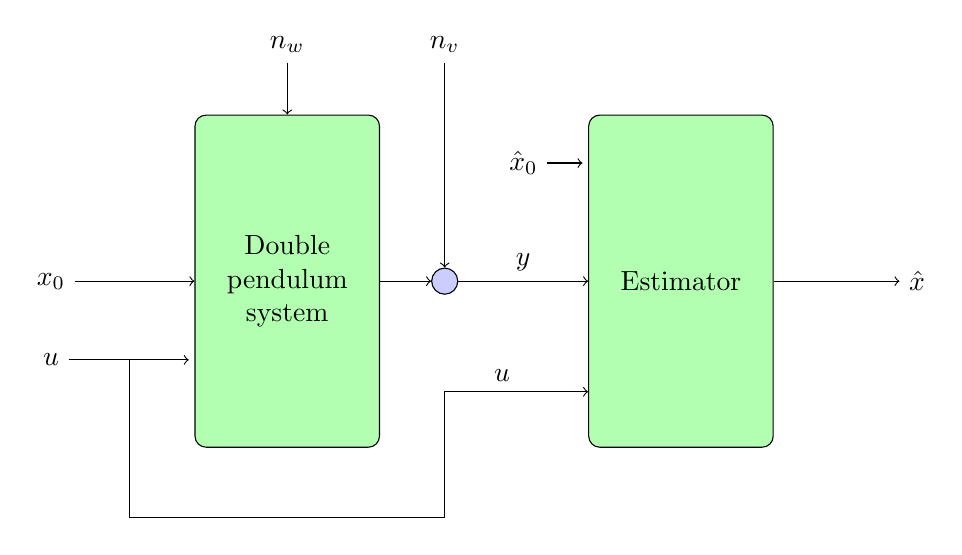
\begin{tikzpicture}
	% Define the nodes in the picture
	\node (sys_in)[yshift=1cm]{$x_0$};
	\node (u_in) [below of=sys_in,node distance=1cm]{$u$};
	\node (sys_u)[input,right of=u_in,node distance=1cm]{};
    \node (sim_sys) [system,right of=sys_in,node distance=3cm] {Double pendulum system};
    \node (sys_noise)[above of=sim_sys,node distance=3cm]{$n_w$};
    \node (msr_noise)[right of=sys_noise,node distance=2cm]{$n_v$};
    \node (msr_add)[sum,right of=sim_sys,node distance=2cm]{};
    \node (estimator) [system,right of=msr_add,node distance =3cm]{ Estimator};
    \node (est_in) [right of=sim_sys,node distance=3cm,yshift=1.5cm]{$\hat{x}_0$};
    \node (est_u) [input,right of =sim_sys, node distance=2cm,yshift=-3cm]{foo};
    \node (est_out)[right of=estimator,node distance=3cm]{$\hat{x}$};
    
    % Define the edges in the picture
    \draw [->] (sys_in) --node{}(sim_sys.west);
    \draw [-] (u_in) --node{}(sys_u);
    \draw [->] (sys_u) --node{}+(\edgedist,0);
    \draw [-] (sys_u) |-node{}(est_u);
    \draw [->] (est_u) |-node[pos=0.7,above]{$u$}(estimator.-130);
    \draw [->] (est_in) --node{}+(\edgedist,0);
    \draw [->] (sys_noise) --node{}(sim_sys.north);
    \draw [->] (msr_noise) --node{}(msr_add.north);
    \draw [->] (sim_sys.east) --node[above]{}(msr_add.west);
    \draw [->] (msr_add.east) --node[above]{$y$}(estimator.west);
    \draw [->] (estimator) --node{}(est_out);
\end{tikzpicture}
    \caption{Experimental setup of inverted double pendulum}
    \label{fig:exp_idp}  
\end{figure}

The state estimation problem is tested using Matlab Simulink. The experimental setup consists of the pendulum system and the state estimator. The pendulum system simulates the dynamical Equations \ref{eq:dyn_idp} of the inverted double pendulum system and outputs the measurements $y$ in Equation \ref{eq:y_idp}. Zero mean Gaussian white noises $n_w$ and $n_v$ are added to the state and measurements equations, so that the simulated system behaves closer to the real system. The state space equations of the pendulum system is 
\begin{equation}
    \label{eq:sim_idp}
    \begin{split}
    \dot x &= f(x,u) + n_w \\
    y &= h(x,u) + n_v,
    \end{split}
\end{equation}
where $n_w$ and $n_v$ are the process and measurement noise. The table below lists the variance of the process and measurement noises used in the experiment.
\begin{table}[H]
    \centering
    \begin{tabular}{|c|c|}
    \hline
    Name of the sensor &Noise variance\\ \hline
    \textbf{Process noise $w_n$:}&\hspace{2mm} \\
    $\dot q_2$ &$1\cdot{10}^{-3}$ \\ \hline
    \textbf{Measurement noise $v_n$:}&\hspace{2mm} \\
     $acc$ &$1\cdot{10}^{-2}$ \\
     $gyro$ &$1\cdot{10}^{-4}$ \\
     $q_2$ &$1\cdot{10}^{-6}$\\ 
     $\dot q_2$ &$1\cdot{10}^{-6}$ \\ \hline
    \end{tabular}
    \caption{ Variance of the Gaussian white noise}
    \label{tab:idp_noise}
\end{table}

%\subsubsection{EKF}
 The equations of continuous time extended Kalman filter is given in Equation \ref{eq:ekf_con}. The non linear state space equation of the system is given in Equations \ref{eq:dyn_ss} and \ref{eq:y_idp}. The Jacobian matrices $A$ and $H$ are computed with the help of symbolic toolbox in Matlab.

In Figure \ref{fig:exp_idp}, $x_0$ and $\hat x_0$ are the initial states of the system and estimator. The input $\tau$ applied is applied to the ankle joint. The initial values of the system are chosen at random. The initial values used in this expreriment is 
$$ x_0 = \begin{bmatrix} 0.9575 \\ 0.9649\\ 0.1576\\ 0.9706 \end{bmatrix}.$$  
The initial values of the state $\hat x_0$ and the covariance matrix $P_0$ is $$P_0 = I_4, \hspace{2cm} \hat x_0 = \textbf{0}_{4,1}$$ where $I_4$ is a $4 \times 4$ identity matrix and $\textbf{0}_{4,1}$ is a column vector of length 4 with all elements as zeros.


The values of the  process covariance $Q$ and measurement covariance $R$ matrices of the EKF are tuned by hand. They are 

$$  \begin{aligned}
    Q&=diag([0; 0; 0; 1\cdot{10}^{-3}]) \\
    R&=diag([1\cdot{10}^{-2}; 1\cdot{10}^{-4}; 1\cdot{10}^{-6}; 1\cdot{10}^{-6}]). \\
    \end{aligned}
    $$

The hand tuned values of the tuning parameters of UKF are 
$$  \begin{aligned}
    \alpha = 1 \\
    \beta = 0\\
    \kappa = -1 
    \end{aligned} $$ 
% Make a plot of the noise and actual measurement data here %
The whole system is simulated for 10 seconds with in 1 millisecond time steps ($\Delta t)$.
\subsubsection{Observation}
\begin{figure}
	\centering
	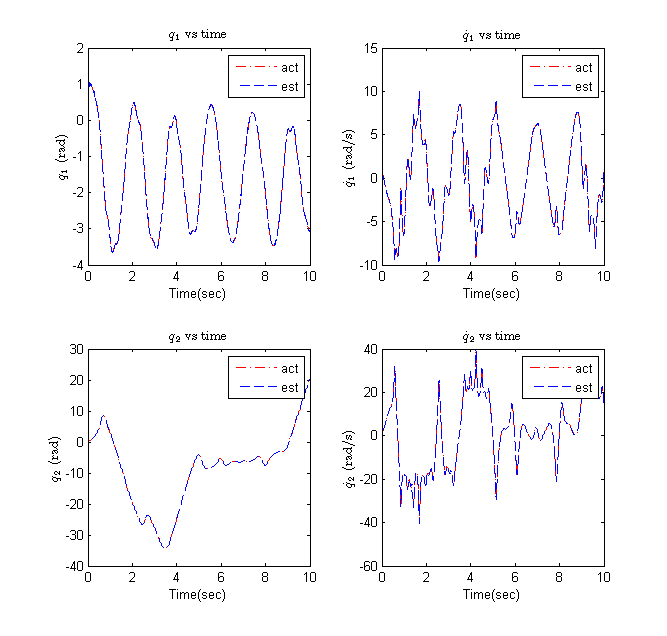
\includegraphics[width=\textwidth, height=0.5\textheight]{Bilder/plots/idp/plot}
%	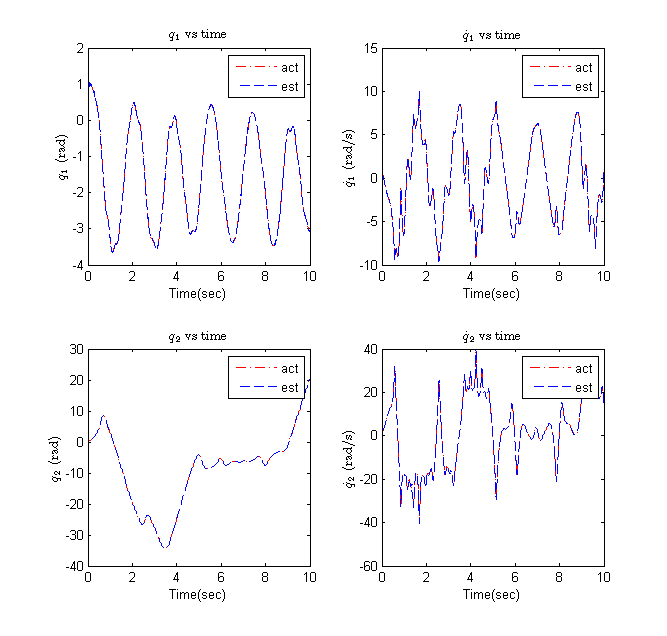
\includegraphics[scale=0.5]{Bilder/plots/idp/plot}
	\caption{ Plots of estimated states $\hat x$ and actual states $x$ vs time}
	\label{fig:idp_plot}
\end{figure}

The estimates $\hat x$ computed by the EKF are plotted in Figures \ref{fig:idp_plot} and \ref{fig:idp_init_conv}. The UKF also produces the estimates similar to EKF. From the plots in Figure \ref{fig:idp_plot} it can be seen that the actual states and estimates converges to same value after some time. 
\begin{figure}
    \centering
       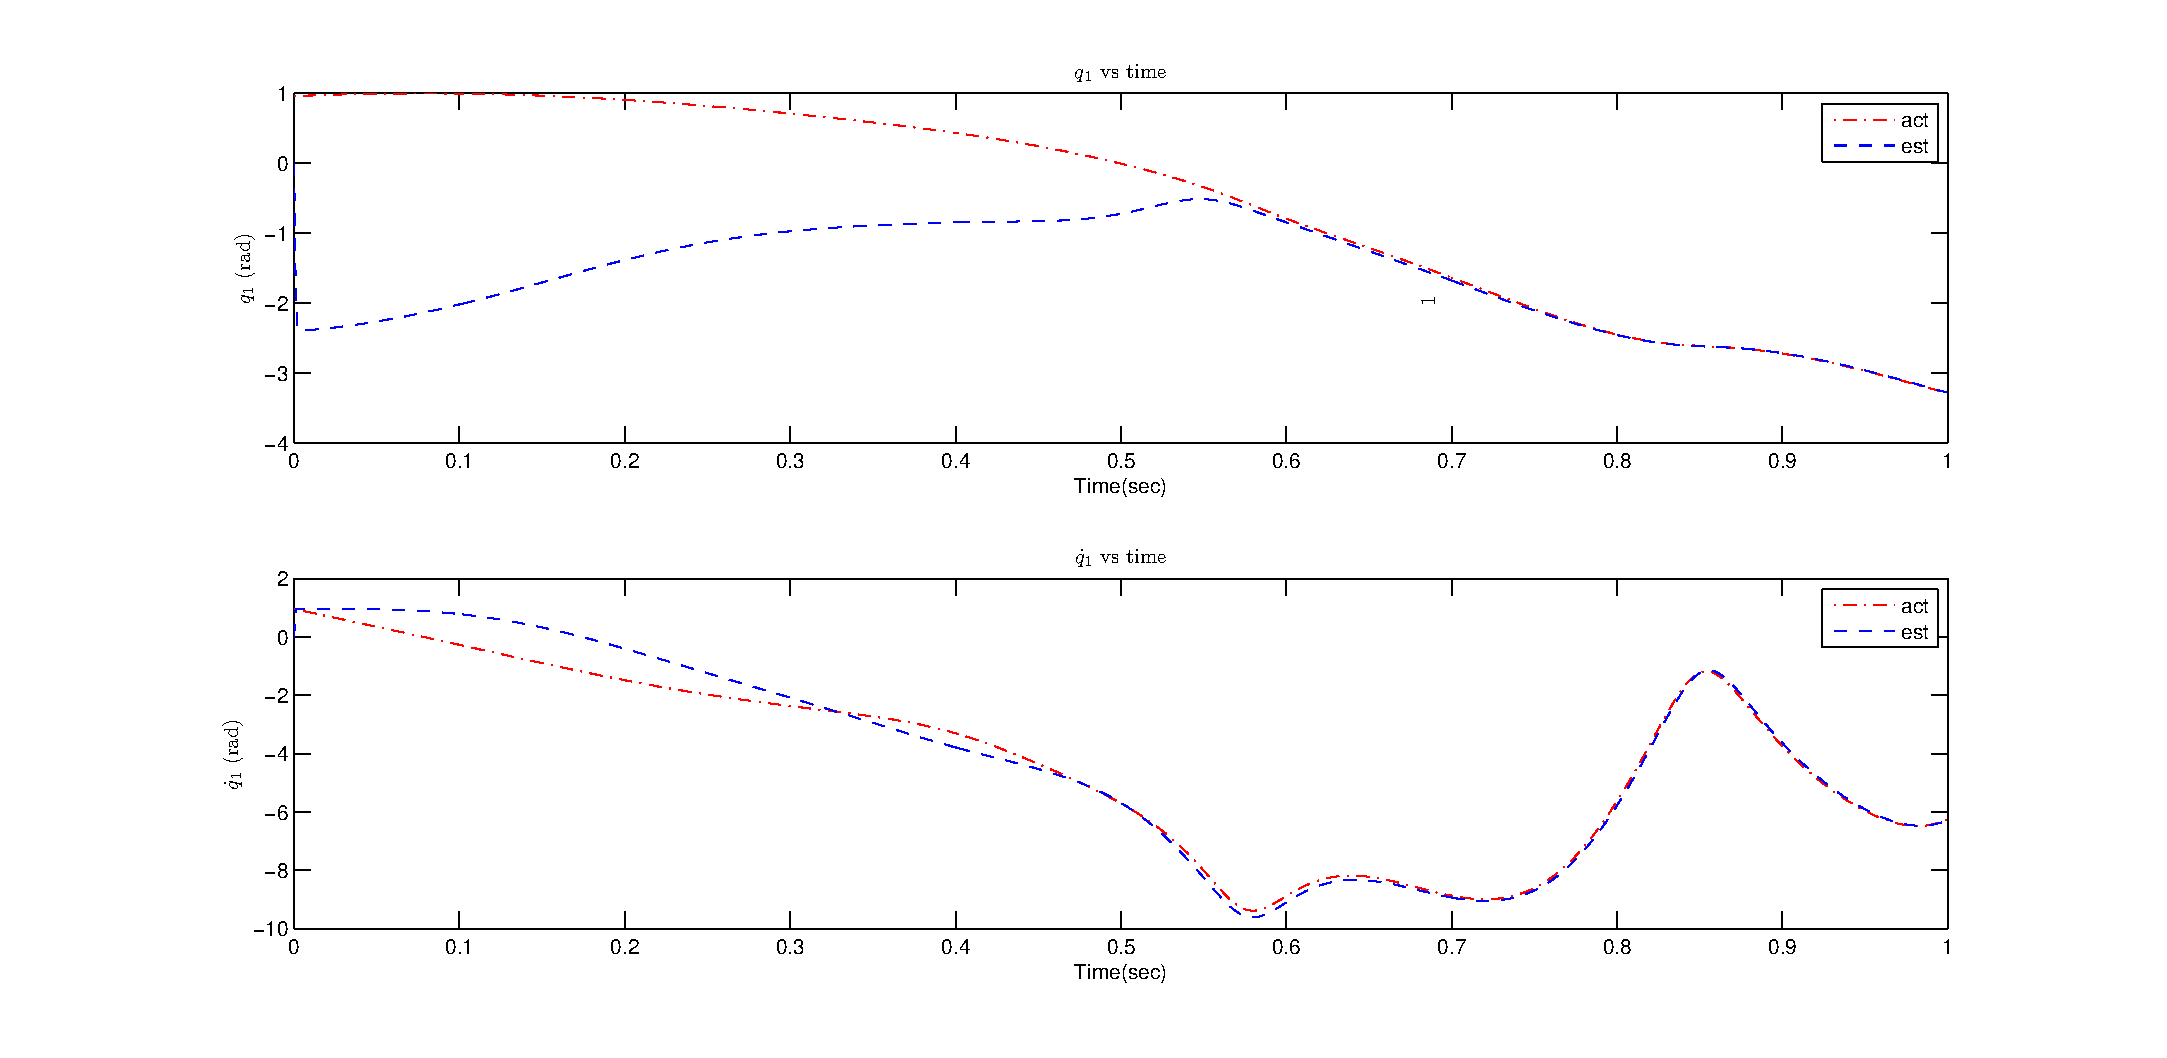
\includegraphics[width=\textwidth, height=0.5\textheight]{Bilder/plots/idp/init_beh}
 %   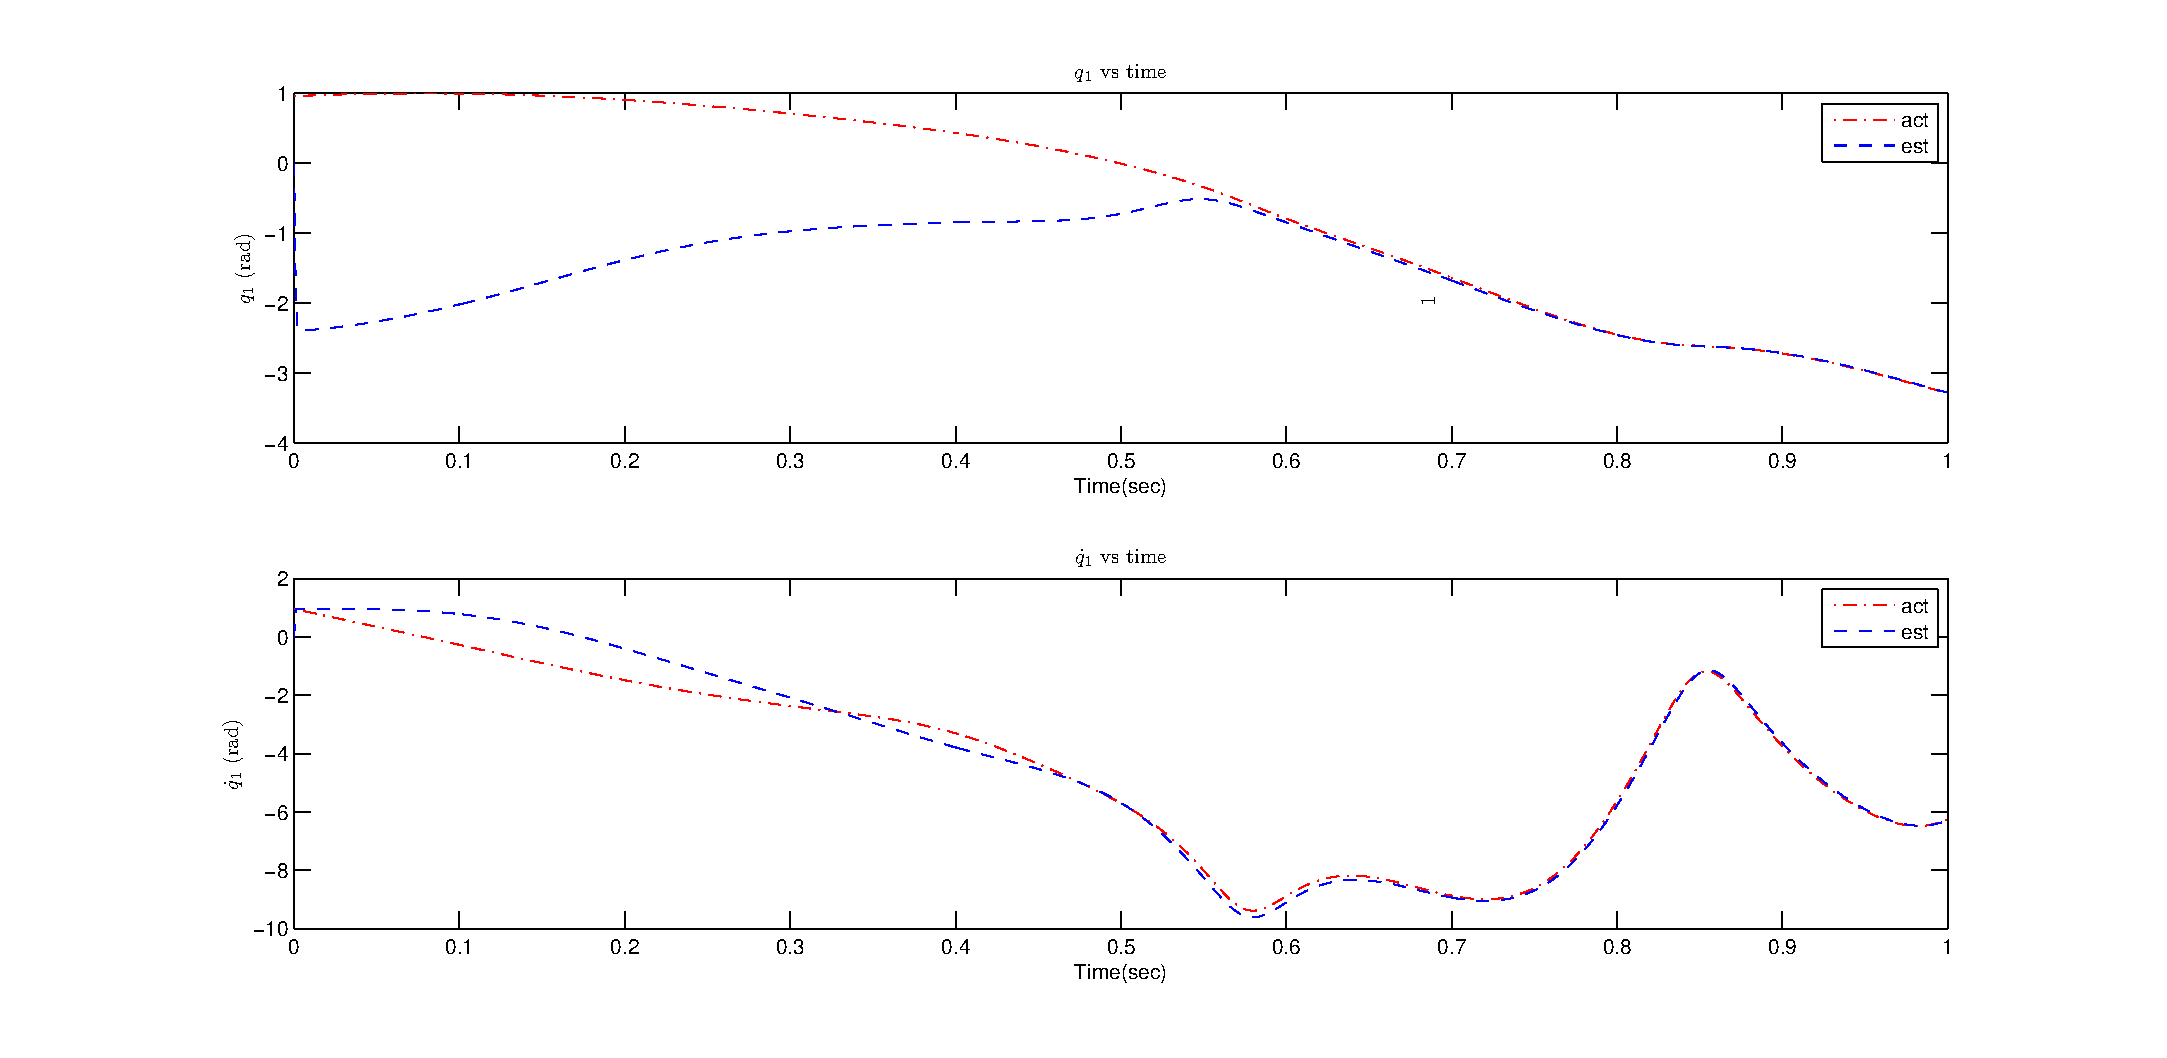
\includegraphics[scale=0.5]{Bilder/plots/idp/init_beh}
    \caption{ Convergence of the estimates $\hat q_1$ and $\hat q_2$ to actual states}
    \label{fig:idp_init_conv}
\end{figure}

The initial convergence of the estimates is shown in Figure \ref{fig:idp_init_conv}. Filter converges in $10ms$ for the given setting of $P_0=I_4$. When the initial error covariance is decreased to $\frac{1}{2}P_0$ the the time taken for convergence increases to $2 sec$. 

\begin{table}[H]
    \centering
    \begin{tabular}{|c|c|}
    \hline
    Estimates &RMSE \\ \hline
    $\hat q_1$   &0.0045 rad \\ \hline
    $\hat {\dot q}_1$ & 0.0261 rad/s \\ \hline
    \end{tabular}
    \caption{RMSE values for EKF estimates}
    \label{tab:idp_rmse_ekf}
\end{table}

\begin{table}[H]
    \centering
    \begin{tabular}{|c|c|}
    \hline
    Estimates &RMSE \\ \hline
    $\hat q_1$   &0.0045 rad \\ \hline
    $\hat {\dot q}_1$ & 0.0332 rad/s\\ \hline
    \end{tabular}
    \caption{RMSE values for UKF estimates}
    \label{tab:idp_rmse_ukf}
\end{table}

\begin{table}[H]
    \centering
    \begin{tabular}{|c|c|}
    \hline
    Estimator &Time(sec) \\ \hline
    $EKF$ &24 \\ \hline
    $UKF$ &30 \\ \hline
    \end{tabular}
    \caption{Time taken for 10 seconds of simulation (simulated with 1ms time steps)}
    \label{tab:idp_sim_time}
\end{table}
The root mean square error (RMSE) value of the states $\hat q_1, \hat{\dot q}_1 $ estimated by EKF and UKF are given in Tables \ref{tab:idp_rmse_ekf} and \ref{tab:idp_rmse_ukf}. Both the UKF and EKF has the same performance in estimating $\hat q_1$ but EKF performs better in estimating $\hat{\dot q}_1$. The time taken for simulation of the EKF is lesser than UKF. The simulation time of UKF depends upon the number of states, as number of sigma points depends upon the number of states. $$\text{Number of sigma points}=2\times \text{Number of states} +1.$$  Moreover the UKF algorithm requries to propogate the sigma points through nonlinear functions twice. In this experiment UKF evaluates the state equations 9 times and the measurement equations 9 times for each time step. But the EKF algorithm evaluates the nonlinear system once per time step. This is the reason for EKF being faster than UKF. 
